\paragraph{Numerical experiments.}
We compare flow-Sinkhorn with vanilla Sinkhorn on the dense geodesic cost matrix, using the previously recorded CPU and GPU runs in Figures~\ref{fig:bench-overview-small} and~\ref{fig:bench-line-gpu-scaling}. The implementations use double precision. The measured quantity is a dual-potential diagnostic, \emph{not} a flow error or the theorem's dual-objective gap. For the centered potential $\widetilde v=v-n^{-1}(\sum_i v_i)\mathbf1$ and a chosen centered LP-optimal potential $\widetilde v^\star$, the recorded statistic is
\begin{equation}\label{eq:benchmark-error}
 e(t)=\min_{s:\ t_s\leq t}\ \min_{\sigma\in\{-1,1\}}
 \frac{\|\widetilde v^{(s)}-\sigma\widetilde v^\star\|_2}
 {\|\widetilde v^\star\|_2}.
\end{equation}
The benchmark code includes the sign alignment to accommodate potential conventions; a sign flip is not an additional gauge of a fixed transport problem. The displayed instances have nonzero denominator. On graphs where the LP potential is nonunique beyond its additive constant, this error depends on the selected reference optimizer. It is therefore an empirical diagnostic, not a distance to the whole optimal set and not a certified cost error. Curves show the best recorded error, so their monotonicity does not assert monotonicity of potential distances along the actual iterates.

The benchmark configurations are:
\begin{itemize}[leftmargin=1.2em,itemsep=2pt,topsep=3pt,parsep=0pt]
\item \textbf{Line.} A path with $n=80$ vertices, $p=158$ directed edges of unit weight, and uniform source and target measures supported on the first and last $m=6$ vertices. GPU runs also use $(n,m)=(160,12),(320,24)$. Here $D_{ij}=|i-j|$ and $W_1=\sum_{i=1}^{n-1}|\sum_{j\leq i}q_j|$, so both ground distances and the reference cost can be computed without Floyd--Warshall or an LP solver.
\item \textbf{Delaunay.} A cloud of $n=140$ points in the unit square, Delaunay edges with Euclidean weights, and uniform measures on $m=7$ points near the upper-left and lower-right corners. The realized edge count depends on the triangulation.
\item \textbf{Single cell.} Waddington-OT single-cell RNA-seq measurements of mouse embryonic fibroblast reprogramming toward pluripotency~\citep{schiebinger2019optimal}. We subsample $60$ cells at each of days $0,0.5,1,1.5$, yielding $n=240$ vertices in a $30$-dimensional PCA representation. A symmetrized $4$-nearest-neighbor graph, with connectivity repair when necessary, carries Euclidean edge costs. Blue and red measures are uniform over the initial and final sampled time points. Flow on this cell-state graph is an illustrative transport proxy for reprogramming trajectories, not a validated reconstruction of lineage or fate, and does not replace the temporal/growth model of Waddington-OT.
\end{itemize}
Graph renderings aggregate the two directed entries on an undirected edge as $f_{ij}+f_{ji}$, retain high-magnitude edges for the orange overlay, and draw the underlying graph in gray. Source and target supports are blue and red. CPU plots use common time and error axes for both methods. GPU line experiments use an NVIDIA Quadro RTX 4000 (8 GB); the public drivers also provide a device switch. These are finite-precision benchmark implementations, including their stabilization and relaxation choices, rather than a test of the exact-arithmetic constants in the theorem.

The aim is to illustrate approach to an unregularized reference across regularization strengths, not compare contraction rates for the same regularized functional: the two methods penalize entropy on different variables. Larger $\gamma$ can give a rapid initial improvement and an earlier bias plateau; smaller $\gamma$ can reduce that bias at higher numerical cost. For machine learning, non-vanishing regularization often improves stability or generalization, so approaching the unregularized solution fastest is not necessarily the relevant downstream objective. An extensive task-based evaluation or comparison with exact flow solvers is beyond these experiments. The figures retain the historical runs; their caption ranges must not be confused with newer screening defaults in the benchmark scripts.

\begin{figure}[htbp]
\centering
\begin{minipage}{0.3\linewidth}\centering
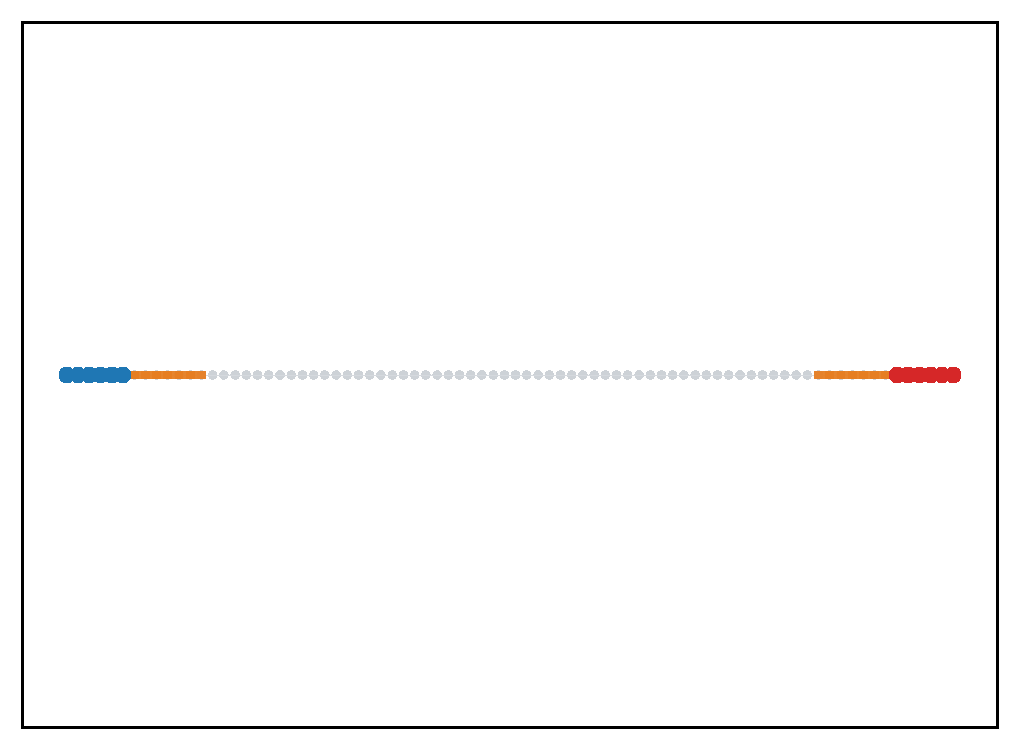
\includegraphics[width=\linewidth]{figures/benchmark-small-line-graph.pdf}
\end{minipage}\hfill
\begin{minipage}{0.3\linewidth}\centering
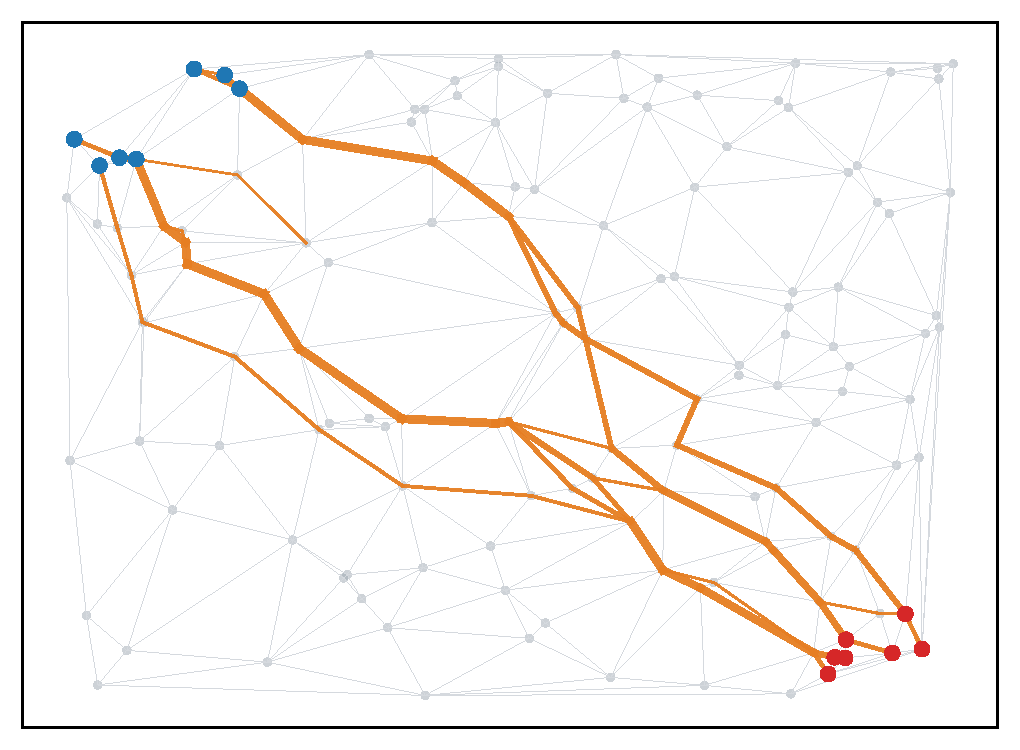
\includegraphics[width=\linewidth]{figures/benchmark-small-delaunay-graph.pdf}
\end{minipage}\hfill
\begin{minipage}{0.3\linewidth}\centering
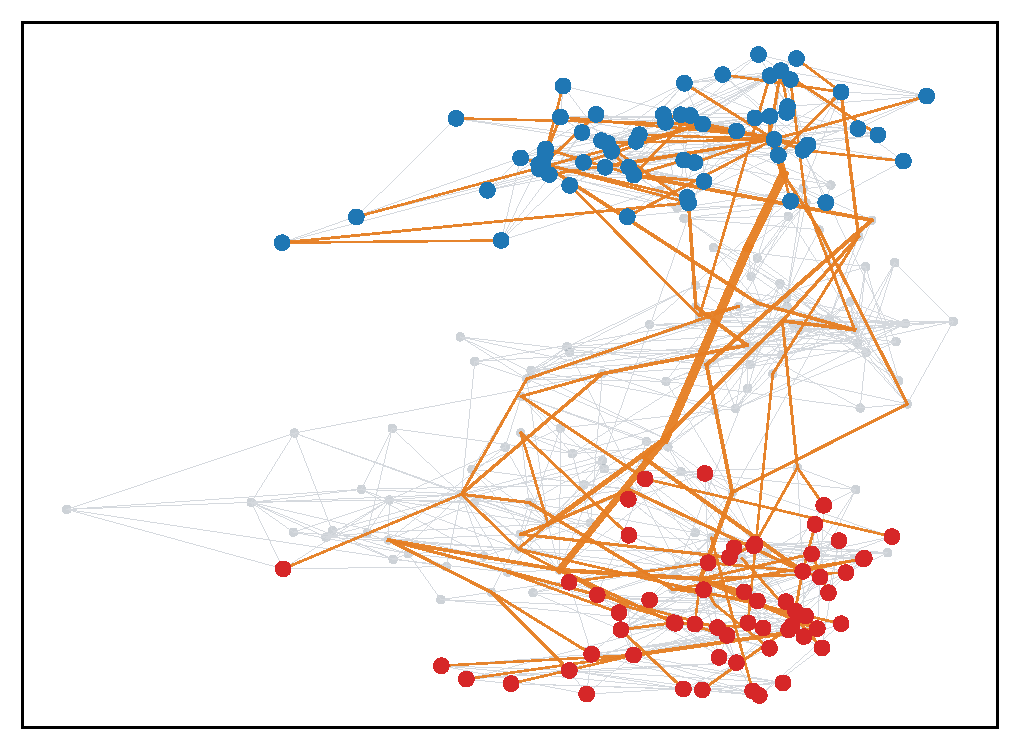
\includegraphics[width=\linewidth]{figures/benchmark-small-singlecell-graph.pdf}
\end{minipage}
% \medskip
\begin{minipage}{0.32\linewidth}\centering
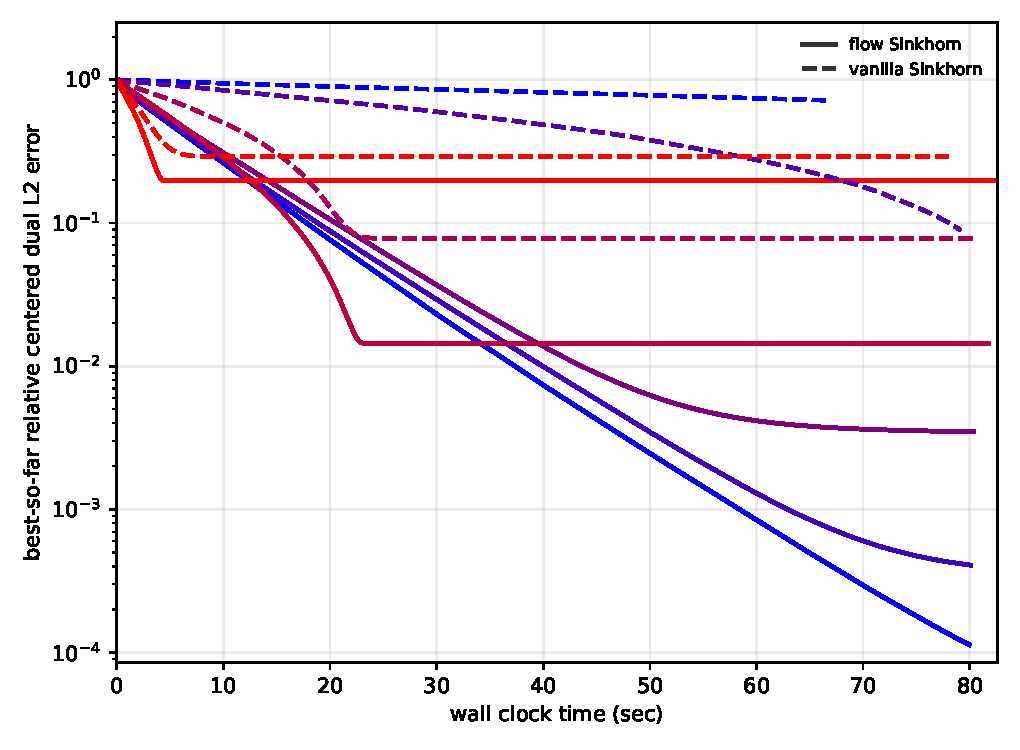
\includegraphics[width=\linewidth]{figures/benchmark-small-line-convergence.pdf}
\end{minipage}\hfill
\begin{minipage}{0.32\linewidth}\centering
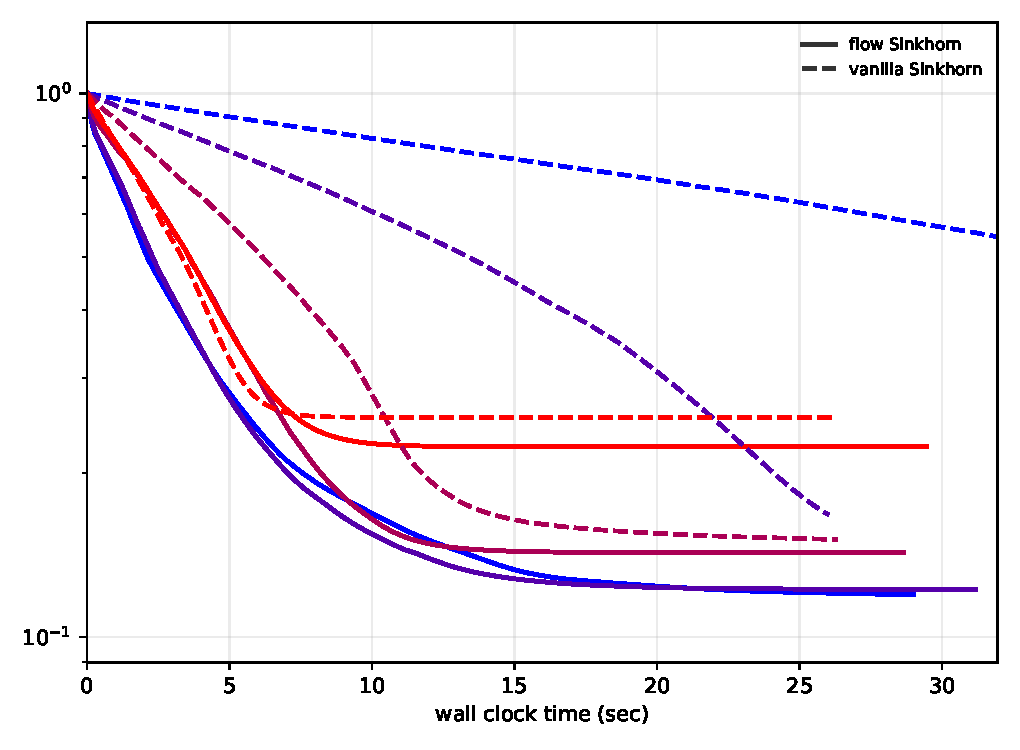
\includegraphics[width=\linewidth]{figures/benchmark-small-delaunay-convergence.pdf}
\end{minipage}\hfill
\begin{minipage}{0.32\linewidth}\centering
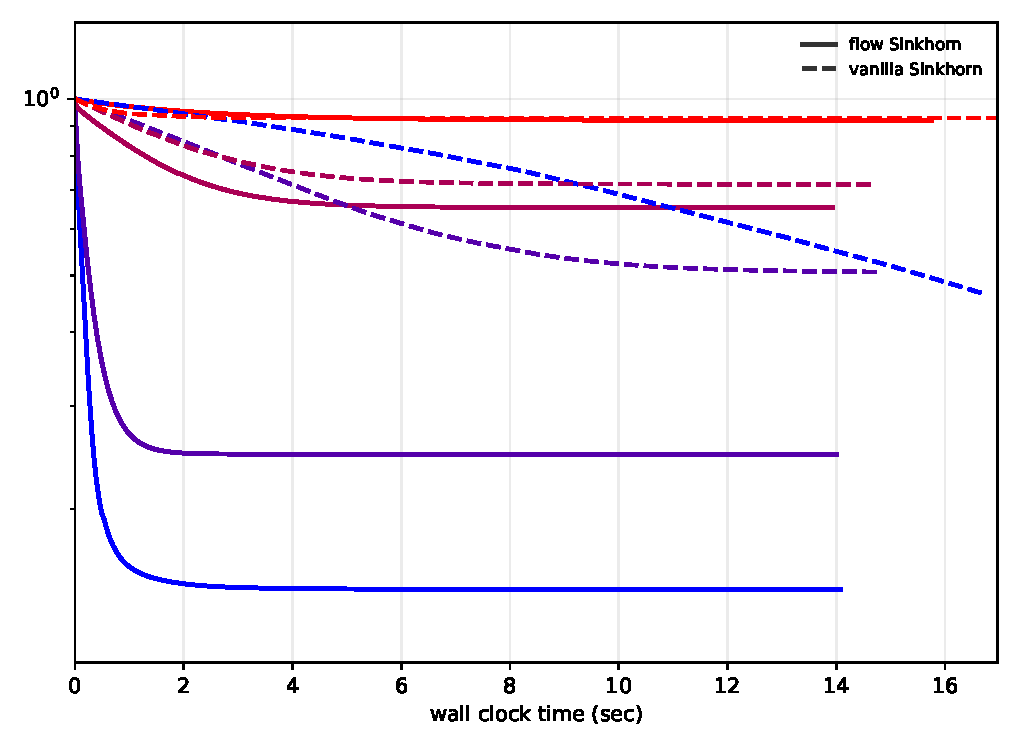
\includegraphics[width=\linewidth]{figures/benchmark-small-singlecell-convergence.pdf}
\end{minipage}\vspace{-2mm}
\caption{Top row: benched graph together with the flow $f$ (line graph, planar Delaunay, single cell). Bottom row: best-so-far relative centered dual-potential error $e(t)$, defined in the text, against wall-clock time. Flow Sinkhorn is plain and vanilla Sinkhorn is dashed; colors encode $\gamma$ from blue (small) to red (large).
Gamma ranges are: line (flow $\gamma\in[10^{-3},5]$, vanilla $\gamma\in[10^{-1},1]$), Delaunay (flow $\gamma\in[9\times10^{-4},9\times10^{-3}]$, vanilla $\gamma\in[9\times10^{-4},9\times10^{-3}]$), single-cell (flow $\gamma\in[3\times10^{-1},9]$, vanilla $\gamma\in[1,5]$).}
\label{fig:bench-overview-small}
\end{figure}

\begin{figure}[htbp]
\centering
\begin{minipage}{0.32\linewidth}\centering
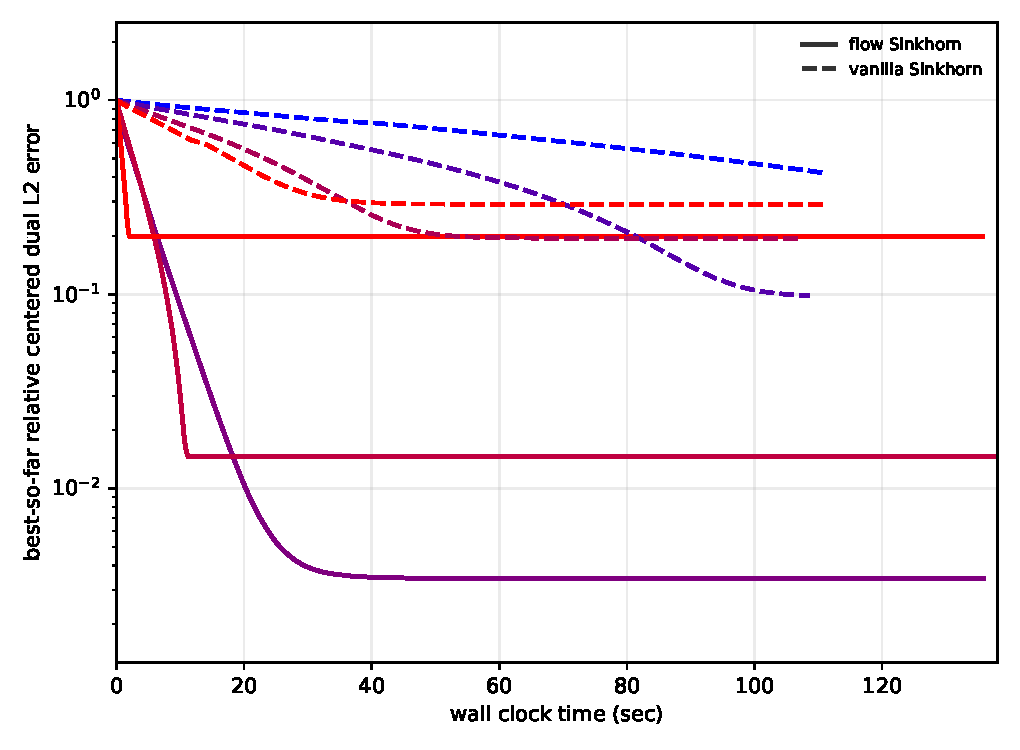
\includegraphics[width=\linewidth]{figures/benchmark-gpu-small-half-tuned-line-convergence.pdf}
\end{minipage}\hfill
\begin{minipage}{0.32\linewidth}\centering
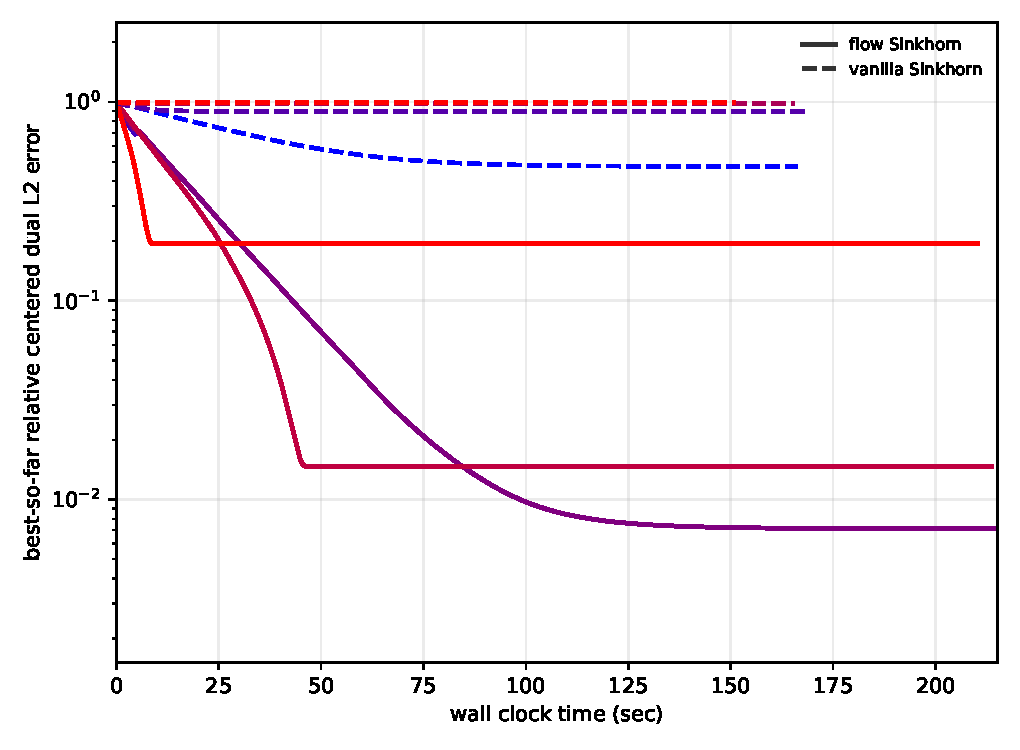
\includegraphics[width=\linewidth]{figures/benchmark-gpu-large-half-tuned-v2-line-convergence.pdf}
\end{minipage}\hfill
\begin{minipage}{0.32\linewidth}\centering
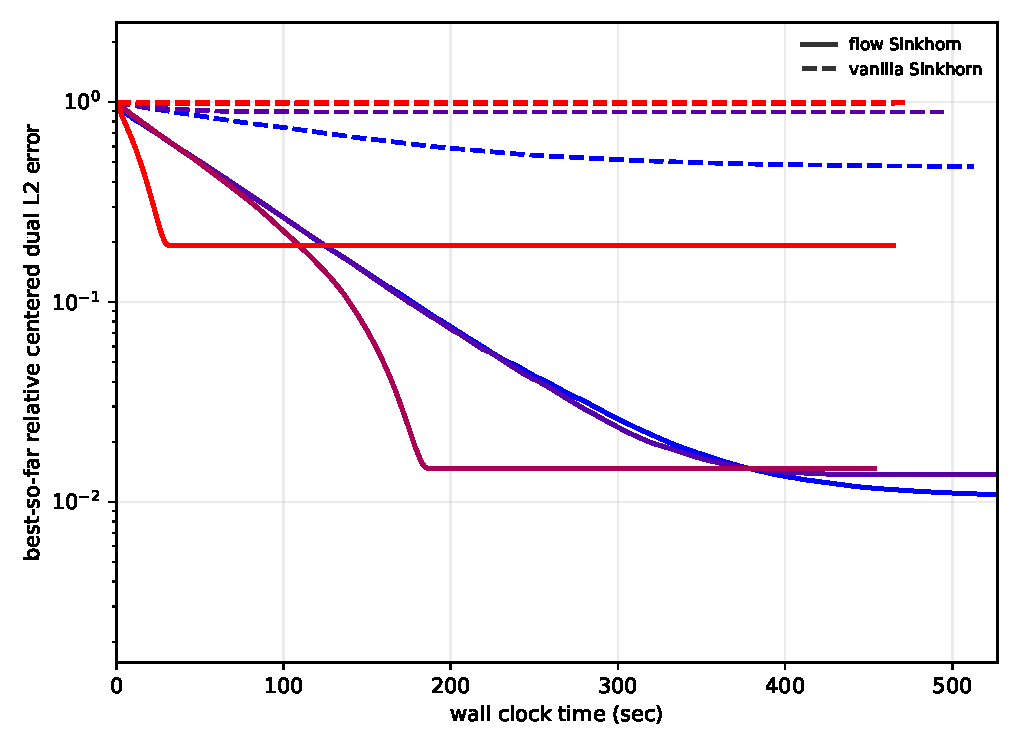
\includegraphics[width=\linewidth]{figures/benchmark-gpu-larger-half-tuned-v6-line-convergence.pdf}
\end{minipage}\vspace{-2mm}
\caption{GPU line-graph benchmark, same best-so-far relative centered dual-potential error as in Figure~\ref{fig:bench-overview-small}. From left to right: small ($n=80,m=6$), large ($n=160,m=12$), and larger ($n=320,m=24$) line-segment tests. %  Flow-Sinkhorn curves are solid and vanilla Sinkhorn curves are dashed.
}
\label{fig:bench-line-gpu-scaling}
\end{figure}
